\documentclass[onecolumn,10pt]{jhwhw}

\usepackage{epsfig} %% for loading postscript figures
\usepackage{amsmath}
\usepackage{graphicx}
\usepackage{grffile}
\usepackage{pdfpages}
\usepackage{algpseudocode}
\usepackage{wrapfig}
\usepackage{booktabs}
\usepackage{multicol}
\usepackage{cancel}
% \usepackage{geometry}
% \geometry{margin=0.75in}

% Default fixed font does not support bold face
\DeclareFixedFont{\ttb}{T1}{txtt}{bx}{n}{12} % for bold
\DeclareFixedFont{\ttm}{T1}{txtt}{m}{n}{12} % for normal

% Custom colors
\usepackage{color}
\usepackage{listings}
\usepackage{framed}
\usepackage{caption}
\usepackage{bm}
\captionsetup[lstlisting]{font={small,tt}}

\author{John Karasinski}
\title{EAE 298 Aeroacoustics \\ Fall Quarter 2016 \\ Homework \#4}

\begin{document}
\maketitle

You are designing a new aircraft engine and analyzing acoustic propagation generated by a non-uniform flow with angle of attack interacting with rotating fans. You obtained flow fields from CFD for a one-sixth small scale of the engine. The radius for the small scale engine is 13 in and the hub radius is 3 in. CFD provides the velocity gust information as a function of its circumferential modes. The circumferential mode for acoustics can be expressed as $m= nB - kV$ where $B$ is the number of blades, $V$ is the number of vanes, $n$ stands for the harmonic of BPF and $k$ is the integer (1, 2, 3$\ldots$). You consider only positive k at this time (this is related the rotation direction of gust). The number of blades is 18. The number of vanes is considered to be 1 since there is no physical vanes but there is one revolution difference. The Mach number is 0.525 and the fan RPM is 8326.3042, the speed of sound is 13503.937009 in/s and the density is 1.4988E-5 slug/in$^3$. The dominant noise is generated at the 1st BPF or n=1 in which the angular frequency is given as $RPM \times \frac{2 \pi}{60} \times B$. We are interested in the propagation through the inlet of the engine so that sound propagates to -z direction assuming the +z direction is in the flow direction.

\problem{[20 points]}
Determine the first five eigenvalues of acoustics for m=18, 17, 16, 15 or (k=1, 2, 3, 4) or (m,n) = (18,0), (18,1), (18,2), (18,3), (18,4), (17,0), (17,1), (17,2), (17,3), (17,4), (16,0), (16,1), (16,2), (16,3), (16,4), (15,0), (15,1), (15,2), (15,3), (15,4)

\begin{figure*}[h]
  \centering
\begin{tabular}{l | rrrr}
\toprule
  &         &         &         &       m \\
n &      15 &      16 &      17 &      18 \\
\midrule
0 &  1.3093 &  1.3895 &  1.4696 &  1.5495 \\
1 &  1.7032 &  1.7896 &  1.8755 &  1.9612 \\
2 &  2.0137 &  2.1036 &  2.1932 &  2.2823 \\
3 &  2.3005 &  2.3932 &  2.4855 &  2.5772 \\
4 &  2.5753 &  2.6702 &  2.7646 &  2.8585 \\
\bottomrule
\end{tabular}
\end{figure*}

\clearpage
\problem{[20 points]}
Plot the five eigenfunctions (radial modes, n=0, 1, 2, 3, 4) for m=18, 17, 16, 15 or (k=1, 2, 3, 4) and verify n describes the number of zero crossings in the radial direction

\begin{figure*}[h]
  \centering
  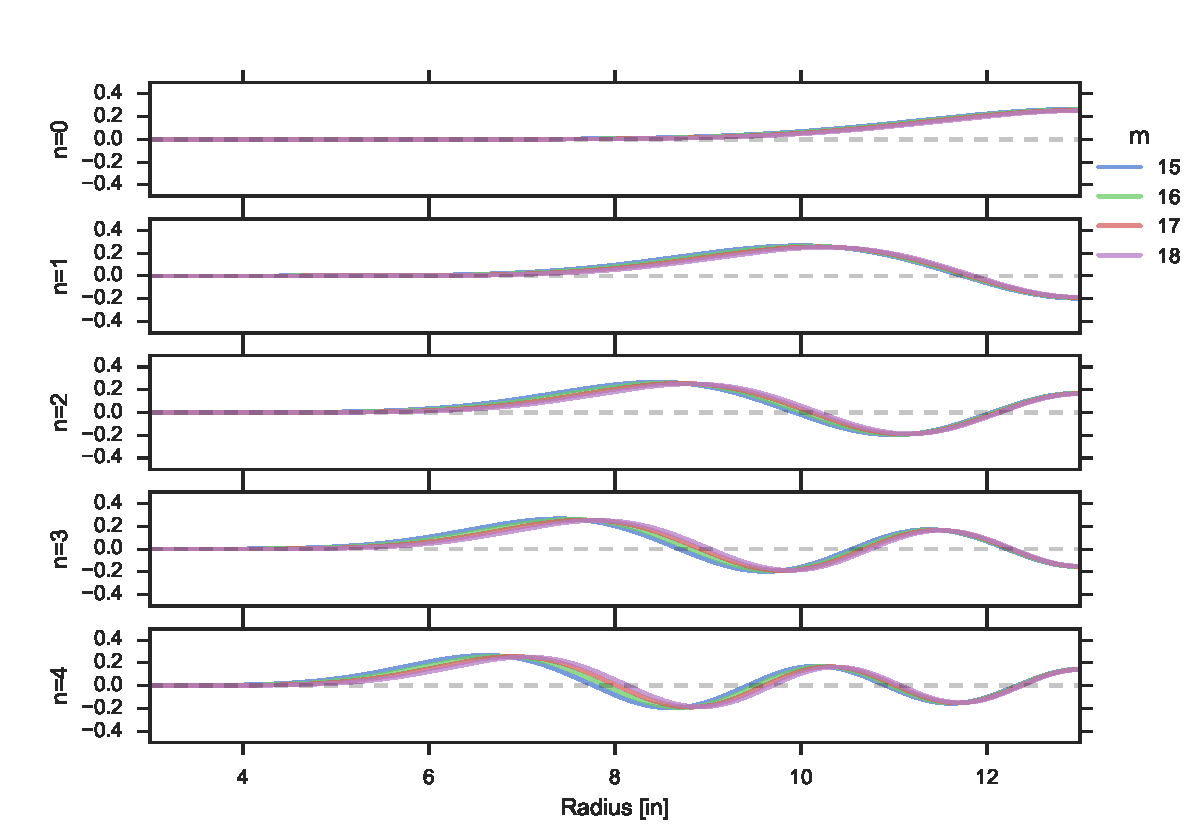
\includegraphics[width=\textwidth]{figs/problem2.pdf}%
  % \caption{The standard narrowband sound pressure level with the reference pressure of 20 micro-Pascal.}%
  % \label{fig:fullfig}%
\end{figure*}

\clearpage
\problem{[20 points]}
Determine the wavenumbers in the z direction for (m,n)=(18,0), (18,1), (18,2), (17,0), (17,1), (17,2), (16,0), (16,1), (16,2), (15,0), (15,1), (15,2). Indicate whether the mode is cut-on (propagating) or cut-off (exponentially decaying). Consider only the propagation in the -z direction. Exclude the exponentially growing solution and include only the propagating solutions or exponentially decaying solutions.

\begin{figure*}[h]
\centering
\begin{tabular}{lr | rr | r r}
\toprule
     m &    n &      $\mu$ &       $K_z$          &  Propagation & Cut\\
\midrule
15 &  0 &  1.3093 & -0.386542 +  0.000000 i &       False  & On  \\
15 &  1 &  1.7032 & -0.842343 +  1.195985 i &       False  & Off \\
15 &  2 &  2.0137 & -0.842343 +  1.738854 i &       False  & Off \\
15 &  3 &  2.3005 & -0.842343 +  2.175252 i &        True  & Off \\
15 &  4 &  2.5753 & -0.842343 +  2.565427 i &        True  & Off \\
16 &  0 &  1.3895 & -0.842343 +  0.301740 i &       False  & Off \\
16 &  1 &  1.7896 & -0.842343 +  1.359038 i &       False  & Off \\
16 &  2 &  2.1036 & -0.842343 +  1.880053 i &       False  & Off \\
16 &  3 &  2.3932 & -0.842343 +  2.309196 i &        True  & Off \\
16 &  4 &  2.6702 & -0.842343 +  2.696039 i &        True  & Off \\
17 &  0 &  1.4696 & -0.842343 +  0.638123 i &       False  & Off \\
17 &  1 &  1.8755 & -0.842343 +  1.510500 i &       False  & Off \\
17 &  2 &  2.1932 & -0.842343 +  2.016453 i &       False  & Off \\
17 &  3 &  2.4855 & -0.842343 +  2.440089 i &        True  & Off \\
17 &  4 &  2.7646 & -0.842343 +  2.824338 i &        True  & Off \\
18 &  0 &  1.5495 & -0.842343 +  0.860357 i &       False  & Off \\
18 &  1 &  1.9612 & -0.842343 +  1.653943 i &       False  & Off \\
18 &  2 &  2.2823 & -0.842343 +  2.148623 i &        True  & Off \\
18 &  3 &  2.5772 & -0.842343 +  2.568059 i &        True  & Off \\
18 &  4 &  2.8585 & -0.842343 +  2.950559 i &        True  & Off \\
\bottomrule
\end{tabular}
\end{figure*}

\clearpage
\problem{[30 points]}
The pressure distribution file at z=0 plane for m=18 or 1 BPF is provided. The first column is the dimensional radius [in], the second column the real part of the pressure [psi], and the third column is the imaginary part of the pressure [psi]. Using this boundary condition, compute the sound power level for (m,n)=(18,0), (18,1), (18,2). This noise is considered for blade self noise that is not associated with the gust response since k=0. Note that the z=0 plane is not the same as the engine inlet. Use the conversion for the unit for the sound power as follows: PWL (dB)=10*log10((Wmn))-10*log10(7.3756E-13)

\end{document}
